\chapter{Desenvolvimento da Solução}
\label{chap:solucaocompleta}

Nesse capítulo será descrito o desenvolvimento da solução. A explicação da solução se embasará no seguinte diagrama de fluxo de dados:

\begin{figure}[h]
	\centering
		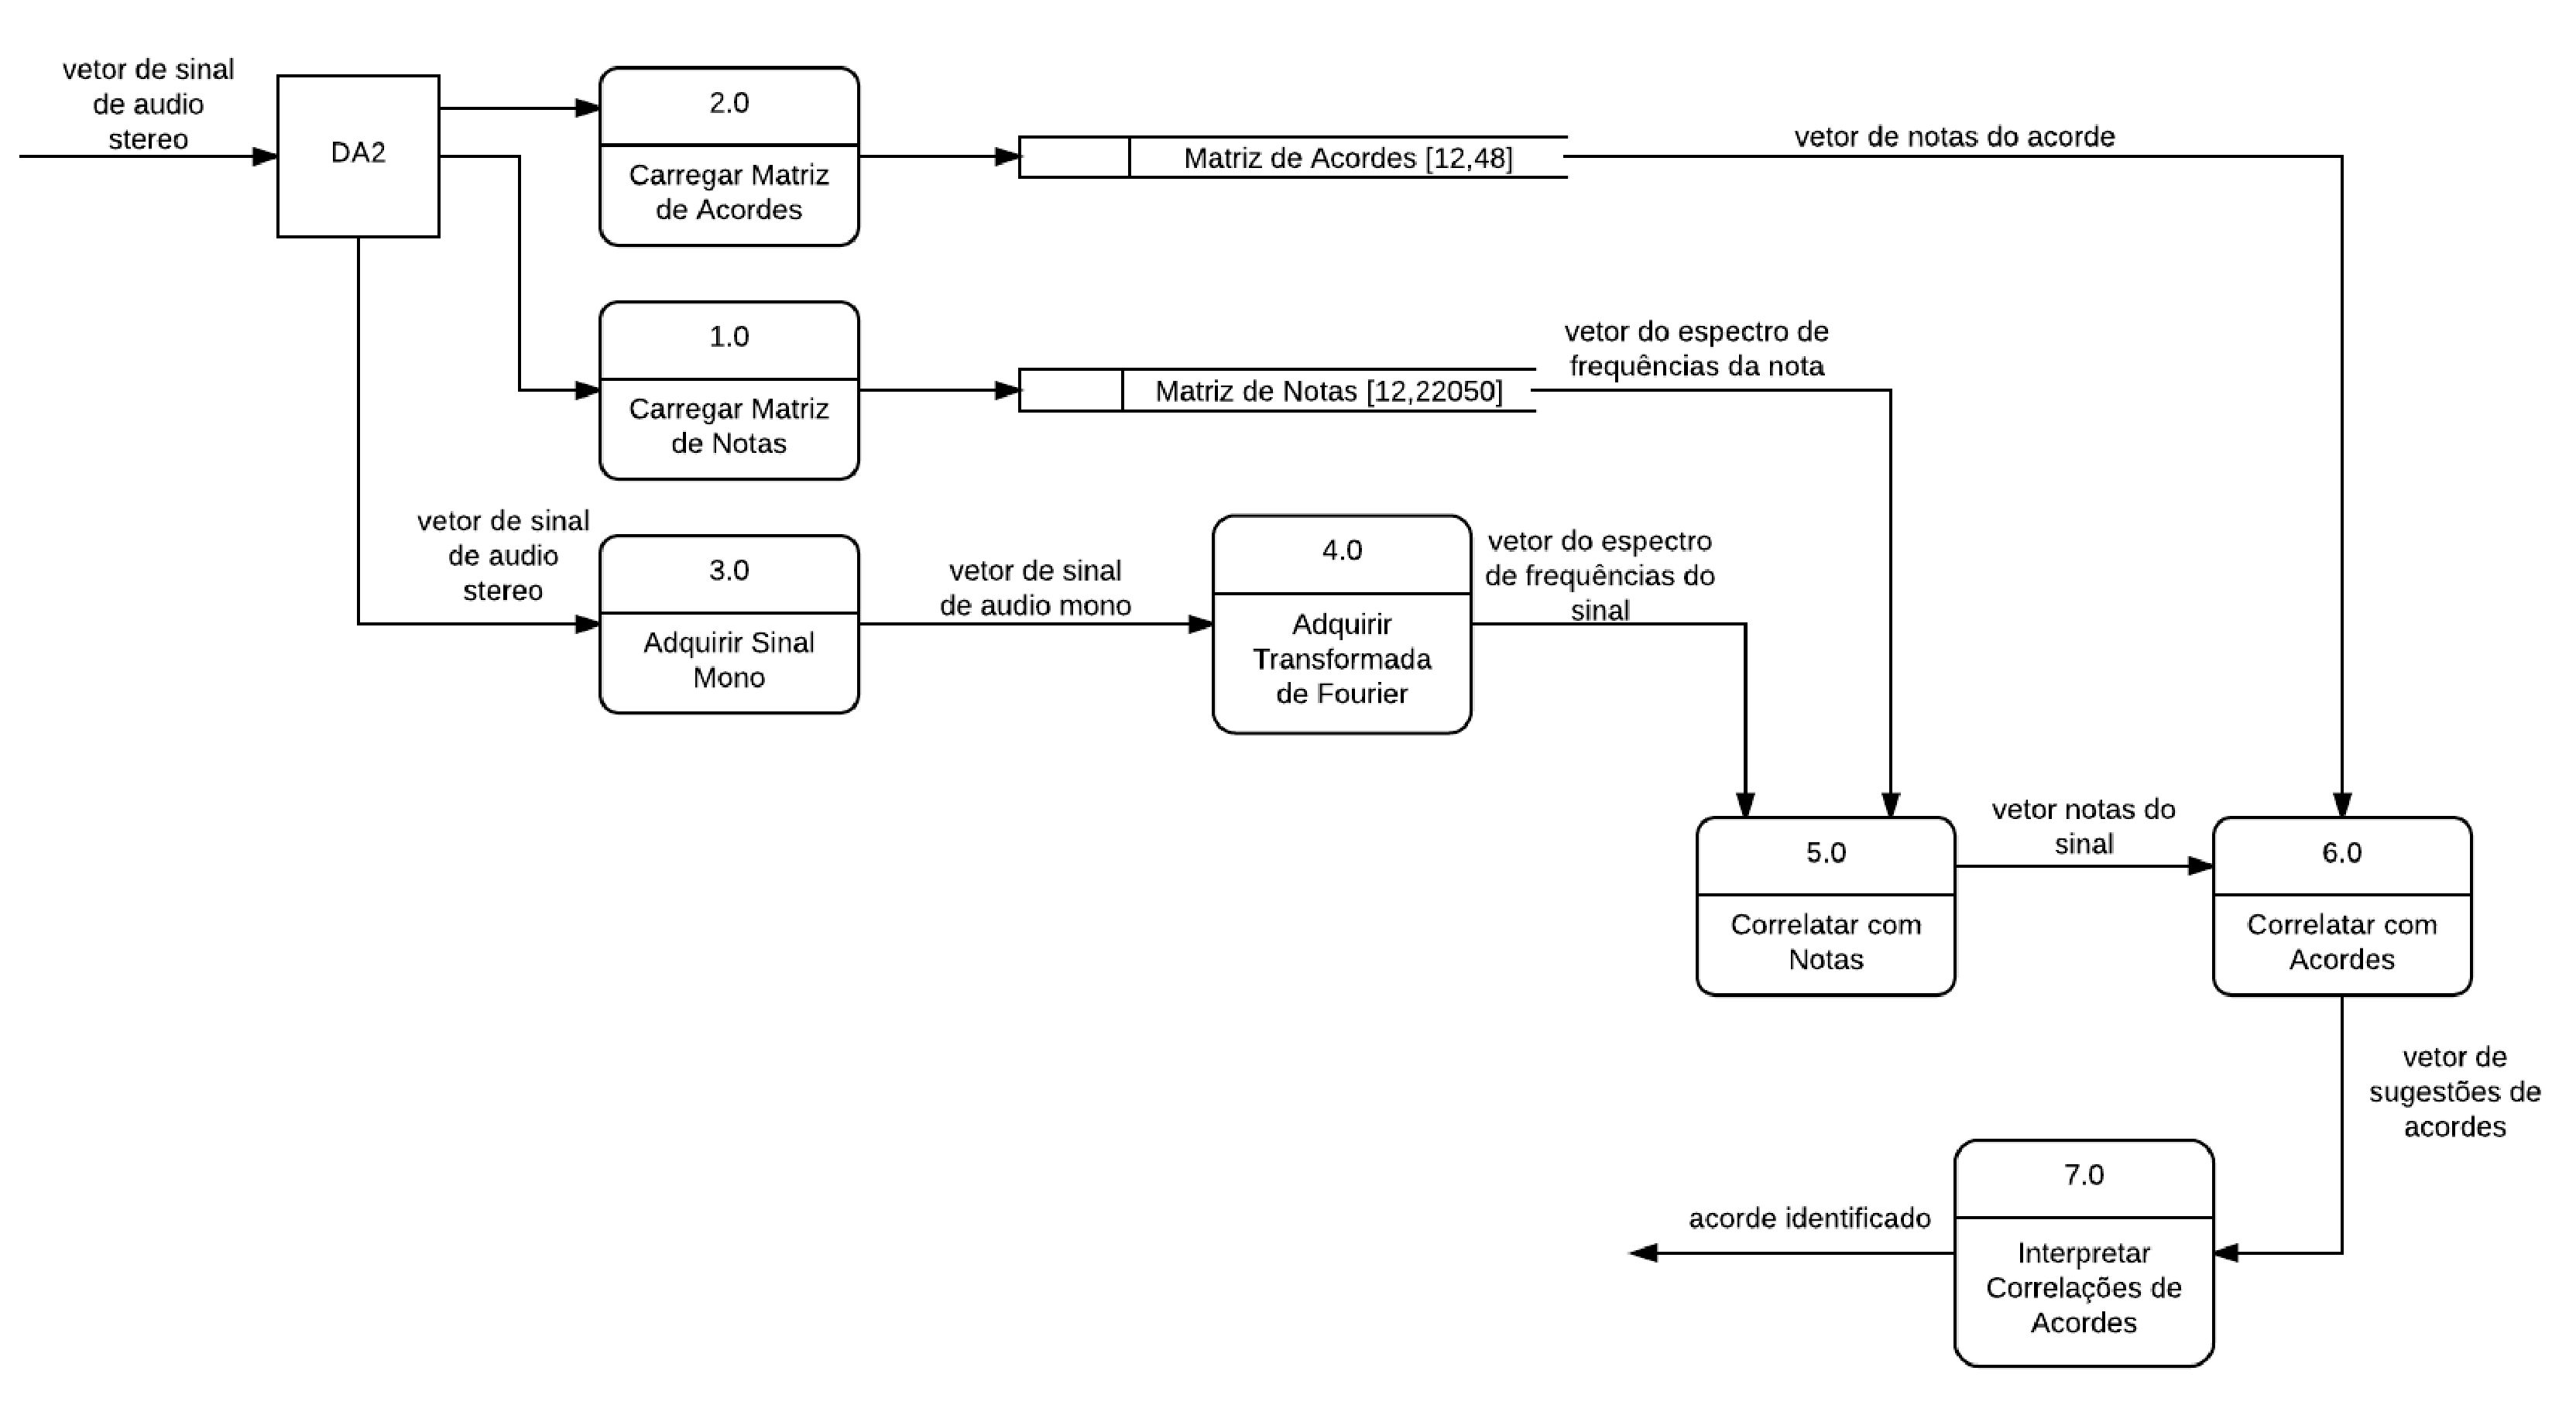
\includegraphics[keepaspectratio=true,scale=0.315]{figuras/dfd.eps}
	\caption{Diagrama de Fluxo de Dados}
\end{figure}

\section{Inicialização do Sistema}
\label{sec:inicializacao}

A solução começa com a chamada da função DA2. Ela recebe como parâmetro um vetor de audio $stereo$, ou seja, ela carrega uma matriz 2 por N, tal que N é o tamanho do sinal de áudio (número de amostras). Esse sinal de áudio é retornado através da função $wavread$($<$$caminho$ $do$ $arquivo$$>$$)$. O tipo de arquivo lido é do formato-padrão de áudio .wav. Esse formato de arquivo permite um armazenamento dos dados em blocos em modulação de pulsos PCM ($pulse-code$ $modulation$). O PCM armazena em arquivo de áudio não-comprimido (sem perdas), ou seja, o processo de amostragem e quantização representa exatamente o que foi descrito na parte de fundamentos teóricos desse trabalho (taxa de amostragem de 44.100 Hz e quantização de 16 bits).

\section{Conversão$stereo$-Mono}
\label{sec:conversao}

Após o sinal ser carregado num vetor de audio$stereo$, ele deverá ser transformado num do tipo mono. Sinal mono de áudio é aquele com somente um canal. Isso é necessário para que o processamento não fosse redundante. Não agregaria valor nesse caso processar um sinal de duplo canal sendo que a fonte emissora de ondas sonoras é comum para ambos. Essa conversão pode ser conferida a seguir:
\begin{lstlisting}
function som = get_mono_signal(som)
	//MONO
	som = som(1:length(som));
	som = som/max(som);
endfunction
\end{lstlisting}

Basicamente a variável de entrada dessa função é reescrita como uma matriz 1 por N, tal qual N é o número de amostras do sinal.

\section{Transformada de Fourier}
\label{sec:transformada}

Após a conversão do sinal para mono canal, o mesmo é submetido há uma transformada de fourier para a obtenção de um vetor no qual cada posição representará um nível de energia para senóides formadoras da onda, funções de bases. O código completo e comentado desse módulo pode ser encontrado na seção de apêndice A.3.

Primeiramente é definido um vetor que representa ao longo da abscissa todas as frequências possíveis - inclusive as que são originadas pela operação de produto interno com a parte complexa da transformada de fourier (o módulo) - dado o conjunto de amostras de áudio:
\begin{lstlisting}
	f = (0 : length(som) - 1) * fs/length(som);
\end{lstlisting}

Porém, como a frequência máxima no espectro é a metade da frequência de amostragem (44.100 Hz), deve-se construir um outro vetor de frequências que vai até no máximo 22.050 Hz:
\begin{lstlisting}
	freq = f(1:round(length(f)/2));
\end{lstlisting}

O passo seguinte é adquirir o módulo da transformada de fourier do sinal. A equação que foi apresentada nesse trabalho foi a DFT. Por motivos de otimização algorítmica, usou-se a FFT (fast fourier transform) que é integrada já ao conjunto de ferramentas do Scilab. O módulo da transformada de fourier é desejável para obter a resposta em frequências do sinal, ou seja, a energia de cada função de base que compõem o sinal. Além disso é desejado um espectro de frequências normalizado e aderente a frequência máxima do áudio (22.050 Hz). Nesse processo não haverá uma parte complexa do sinal. Segue trexo do código:
\begin{lstlisting}
	SOM = abs(fft(som));
	SOM = SOM/max(SOM);
	SOM = SOM(1:round(length(f)/2));
\end{lstlisting}

Depois desse processo há 2 vetores que compõem a representação do módulo espectral, ambos com tamanho igual a metade da quantidade de amostras do sinal original: vetor de frequências e vetor do módulo da transformada de fourier. É desejável para o andamento do processo um vetor de módulo frequencial com o tamanho de 22.050 posições. Esse tamanho é necessário para representar a energia da função de base (senóide) somente acessando a posição do vetor, por exemplo: para saber qual a energia da onda senoidal de 440 Hz é só acessar a posição 440 desse mesmo vetor. Para tal construiu-se o seguinte código:
\begin{lstlisting}
	i = 1;
	j = 0;
	l = 1;
	SOMA = 0;
	while (i<length(freq))
    	if (round(freq(i)) == round(freq(i+1)))
        	SOMA = SOM(i+1) + SOMA;
        	j = j + 1;
   	 	else
        	respfreq(l) = SOMA/(j+1);
        	j = 0;
        	SOMA = SOM(i+1);
        	l = l+1;
    	end
    	i = i+1;
	end
\end{lstlisting}

A variável \textbf{i} representa um iterador para todas as posições do vetor das frequências. A variável \textbf{j} representa uma faixa de frequências, que arredondando as mesmas, são equivalentes. A variável \textbf{l} representa a quantidade total de faixas de frequências, que arredondando as mesmas, são equivalentes de tal forma que \textbf{l}x\textbf{j} = \textbf{i}. A variável \textbf{SOMA} possui a responsabilidade de popular a energia dessas frequências congruentes em cada posição do novo vetor. Esse laço de repetição vai passar pela totalidade das frequências e em cada posição verificará as frequências equivalentes via arredondamento. A medida que se vai encontrando determinadas frequências congruentes, uma posição do valor de energia da transformada de fourier é somada. Quando a próxima frequência não é mais congruente com a anterior, o vetor \textbf{respfreq} recebe a média ponderada dessas energias.

O resultado desse processamento é ilustrado a seguir:

\begin{figure}[h]
	\centering
		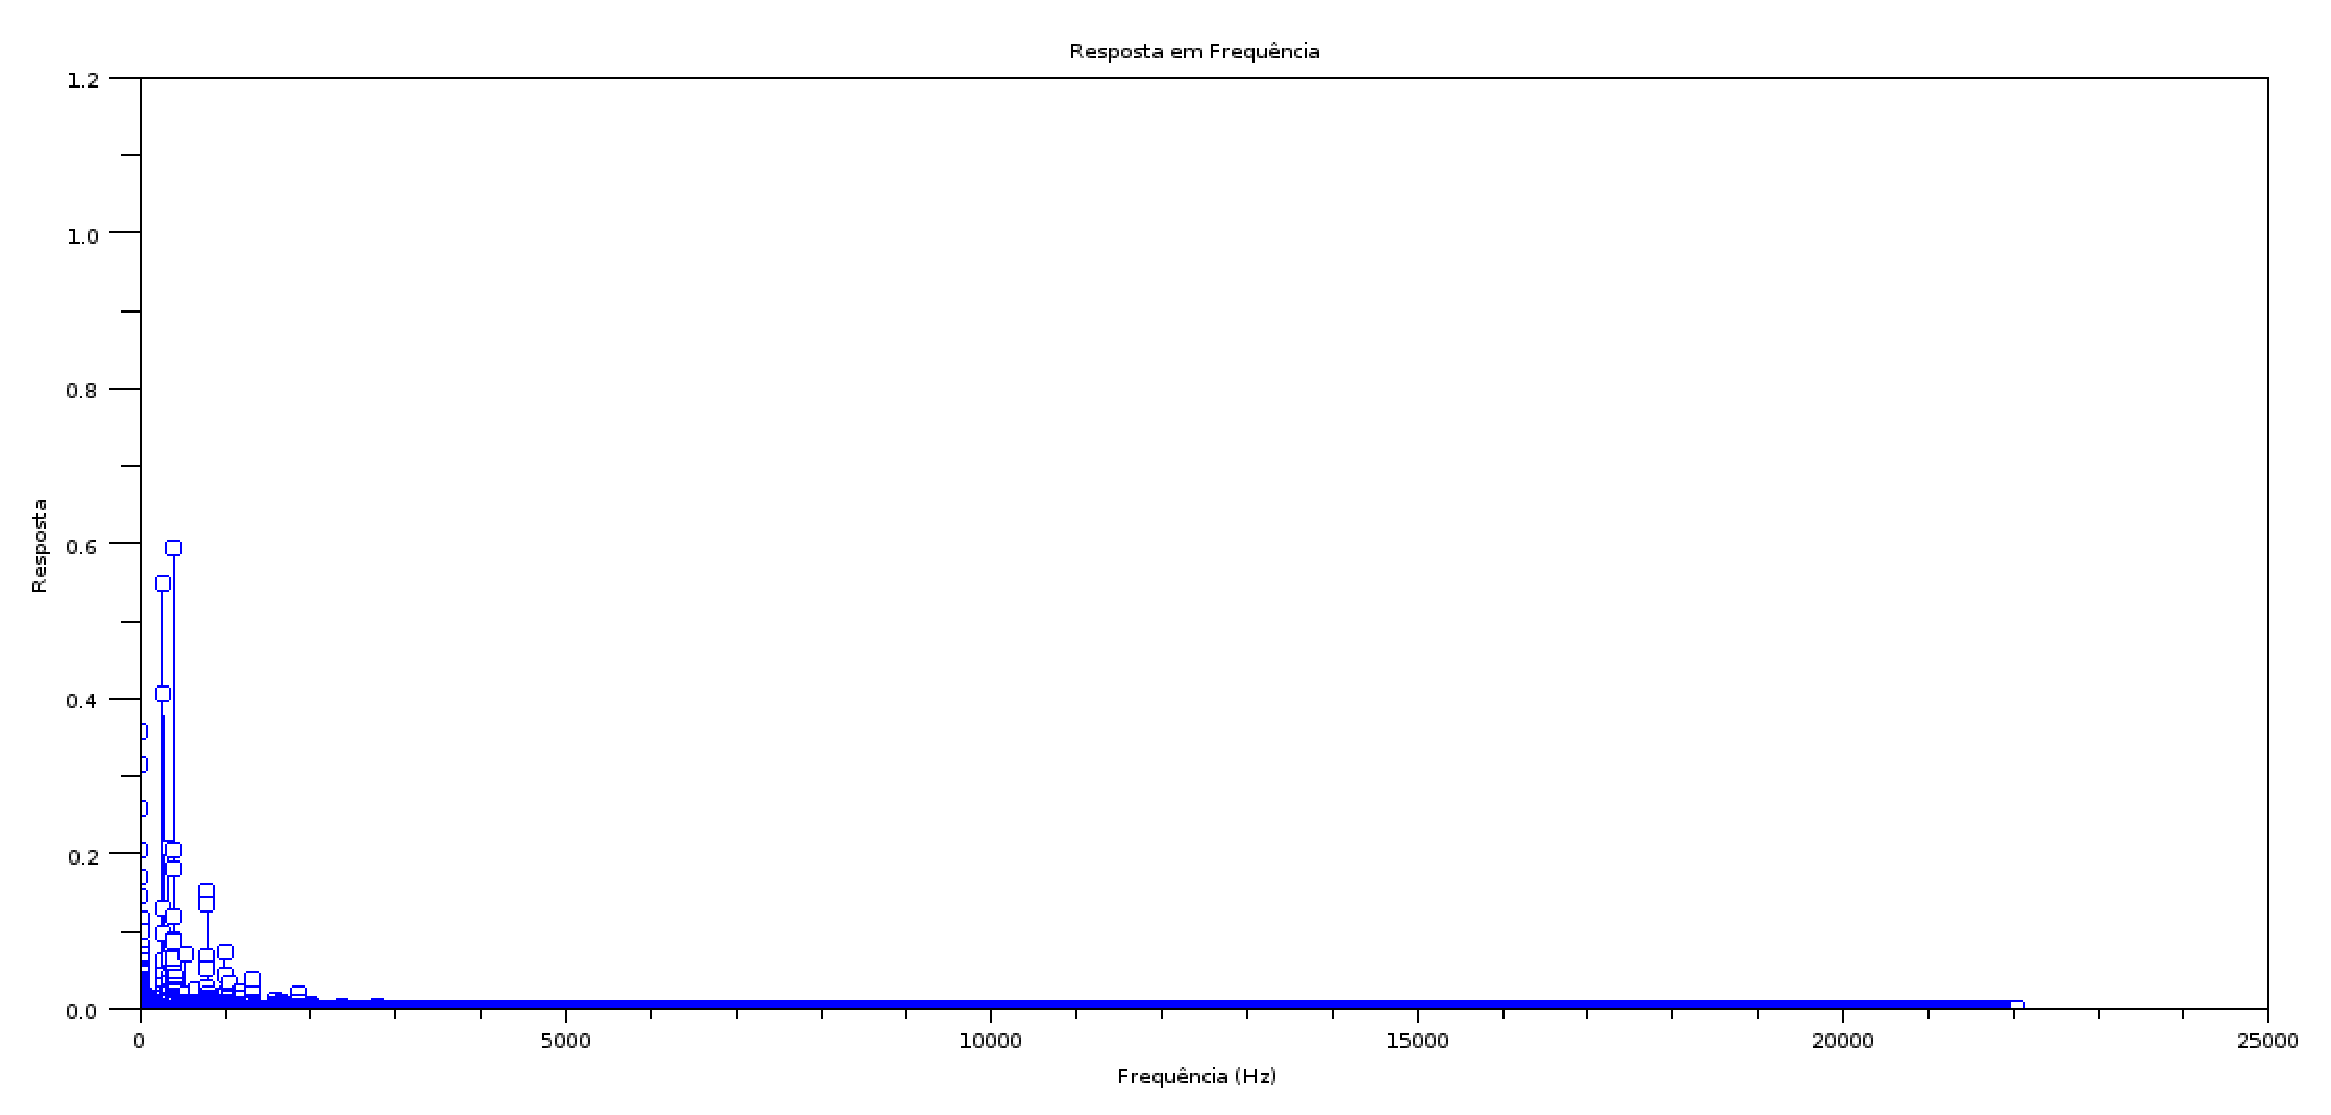
\includegraphics[keepaspectratio=true,scale=0.45]{figuras/fft-resultado}
	\caption{Vetor de 22.050 posições de Resposta em Frequência}
\end{figure}

O espectro de frequências está mais concentrado no lado esquerdo de todos os valores de frequências possíveis e audíveis ao ouvido humano. Esse fato é explicado devido ao uso de notas musicais serem usadas normalmente de 60 Hz a 3000 Hz.

\newpage
\section{Correlação com Notas Musicais}
\label{sec:correlacaonotas}

Na função de correlacionar o espectro de frequência com as notas musicais há a presença de uma estrutura de uma rede neural. Para essa rede foram criados 12 neurônios, 1 para cada nota musical. Segue um exemplo de esquema de um neurônio para a nota $Dó$, para as outras notas segue a mesma estrutura de neurônio:

\begin{figure}[h]
	\centering
		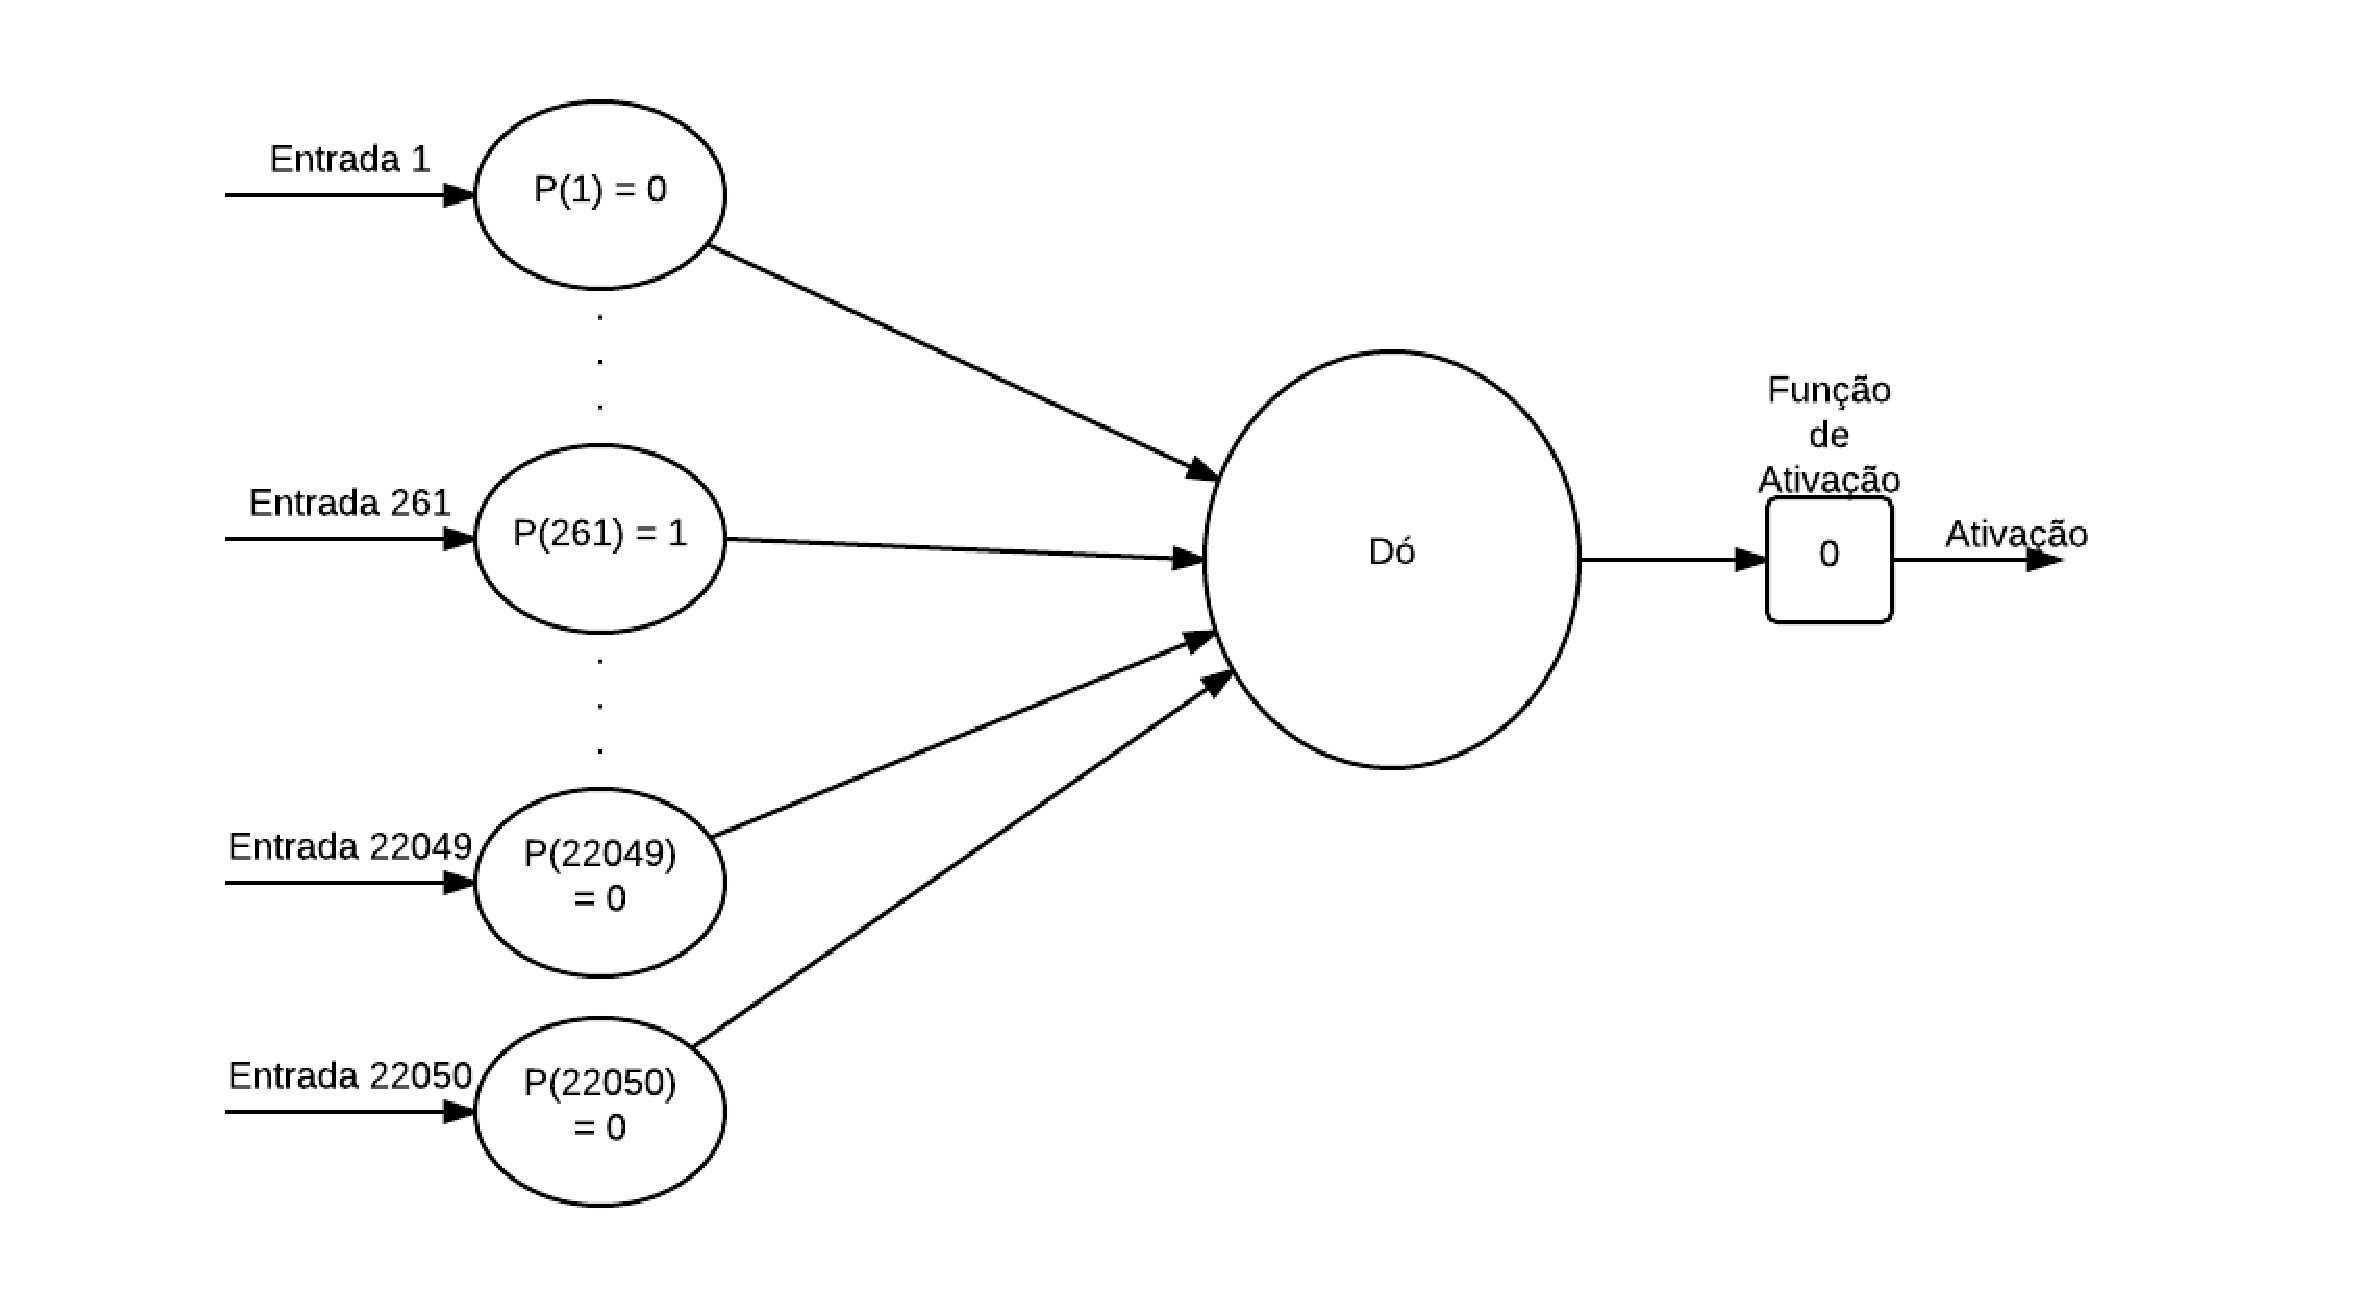
\includegraphics[keepaspectratio=true,scale=0.41]{figuras/neuron_notes}
	\caption{Esquema de Neurônio para Notas}
\end{figure}

Como é mostrado na figura, os neurônios para notas musicais possuem 22050 entradas respectivas a cada frequência. Para cada nota musical há certos pesos diferentes para certas frequências. Os pesos foram obtidos com aprendizagem não-supervisionada, ou seja, não houve nenhum algorítmo de treinamento para a rede. Os pesos foram obtidos por resultados empíricos e são referenciados na seção A.9 dos Apêndices. Os mesmos são gerados no processo de carregar notas.

Para a função de transferência, foi usada a equação de correlação tal qual $x$ é o neurônio constituinte de pesos e $y$ o espectro de frequência do sinal \cite{correlacao}:

\begin{figure}[h]
	\centering
		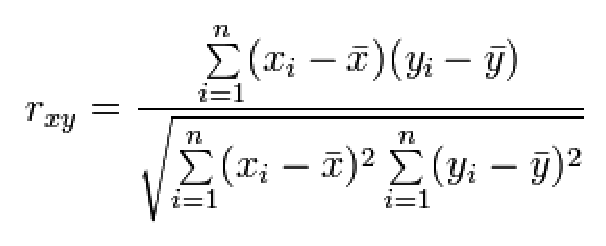
\includegraphics[keepaspectratio=true,scale=0.7]{figuras/correlation-formula}
	\caption{Equação de Correlação}
\end{figure}

Quanto a função de ativação, ela se manteve $f(x)$ $=$ $x$ por motivos de simplificação da aplicação
. Portanto ela é zero, nula ou inexistente.

Para a implementação dessa rede de 12 neurônios segue o código:
\begin{lstlisting}
function S1 = correlate_with_notes(rfeq)
	exec correlation.sci;
	i = 1;
	while (i <= 12)
	    correlacao = coeffcorr(rfeq,notas(i,:));
	    S1(i) = correlacao;
	    i = i + 1;
	end
endfunction
\end{lstlisting}

A função de correleção é nativa do Scilab mas para propósitos didáticos ela está referenciada nos apêndices seção A.6. Nessa estrutura de laço foi calculado cada pontecial de ativação de cada neurônio em relação ao espectro de frequência e guardados na variável \textbf{S1}. Tal vetor pode ser chamado de notas sugeridas.

\section{Correlação com Acordes Musicais}
\label{sec:correlacaoacordes}

Na função de correlacionar as notas musicais sugeridas com acordes há a presença de uma outra estrutura de rede neural. Para essa rede foram criados 48 neurônios, 1 para cada possibilidade de acorde em tríade. Um exemplo de esquema de um neurônio é para o acorde $CM$.

Os neurônios para acordes musicais possuem 12 entradas respectivas a cada nota musical. Para cada acorde musical há certos pesos diferentes para certas notas. Os pesos foram obtidos com aprendizagem não-supervisionada, ou seja, não houve nenhum algorítmo de treinamento para a rede. Os pesos foram obtidos por resultados empíricos e são referenciados na seção A.10 dos Apêndices. Os mesmos são gerados no processo de carregar acordes. Quanto a função de ativação, ela se manteve $f(x)$ $=$ $x$ por motivos de simplificação da aplicação. Portanto ela é zero, nula ou inexistente.

Para a função de transferência, foi usada a mesma equação de correlação para notas musicais. Segue figura ilustrativa do neurônio para o exemplo do acorde de $CM$:

\begin{figure}[t]
	\centering
		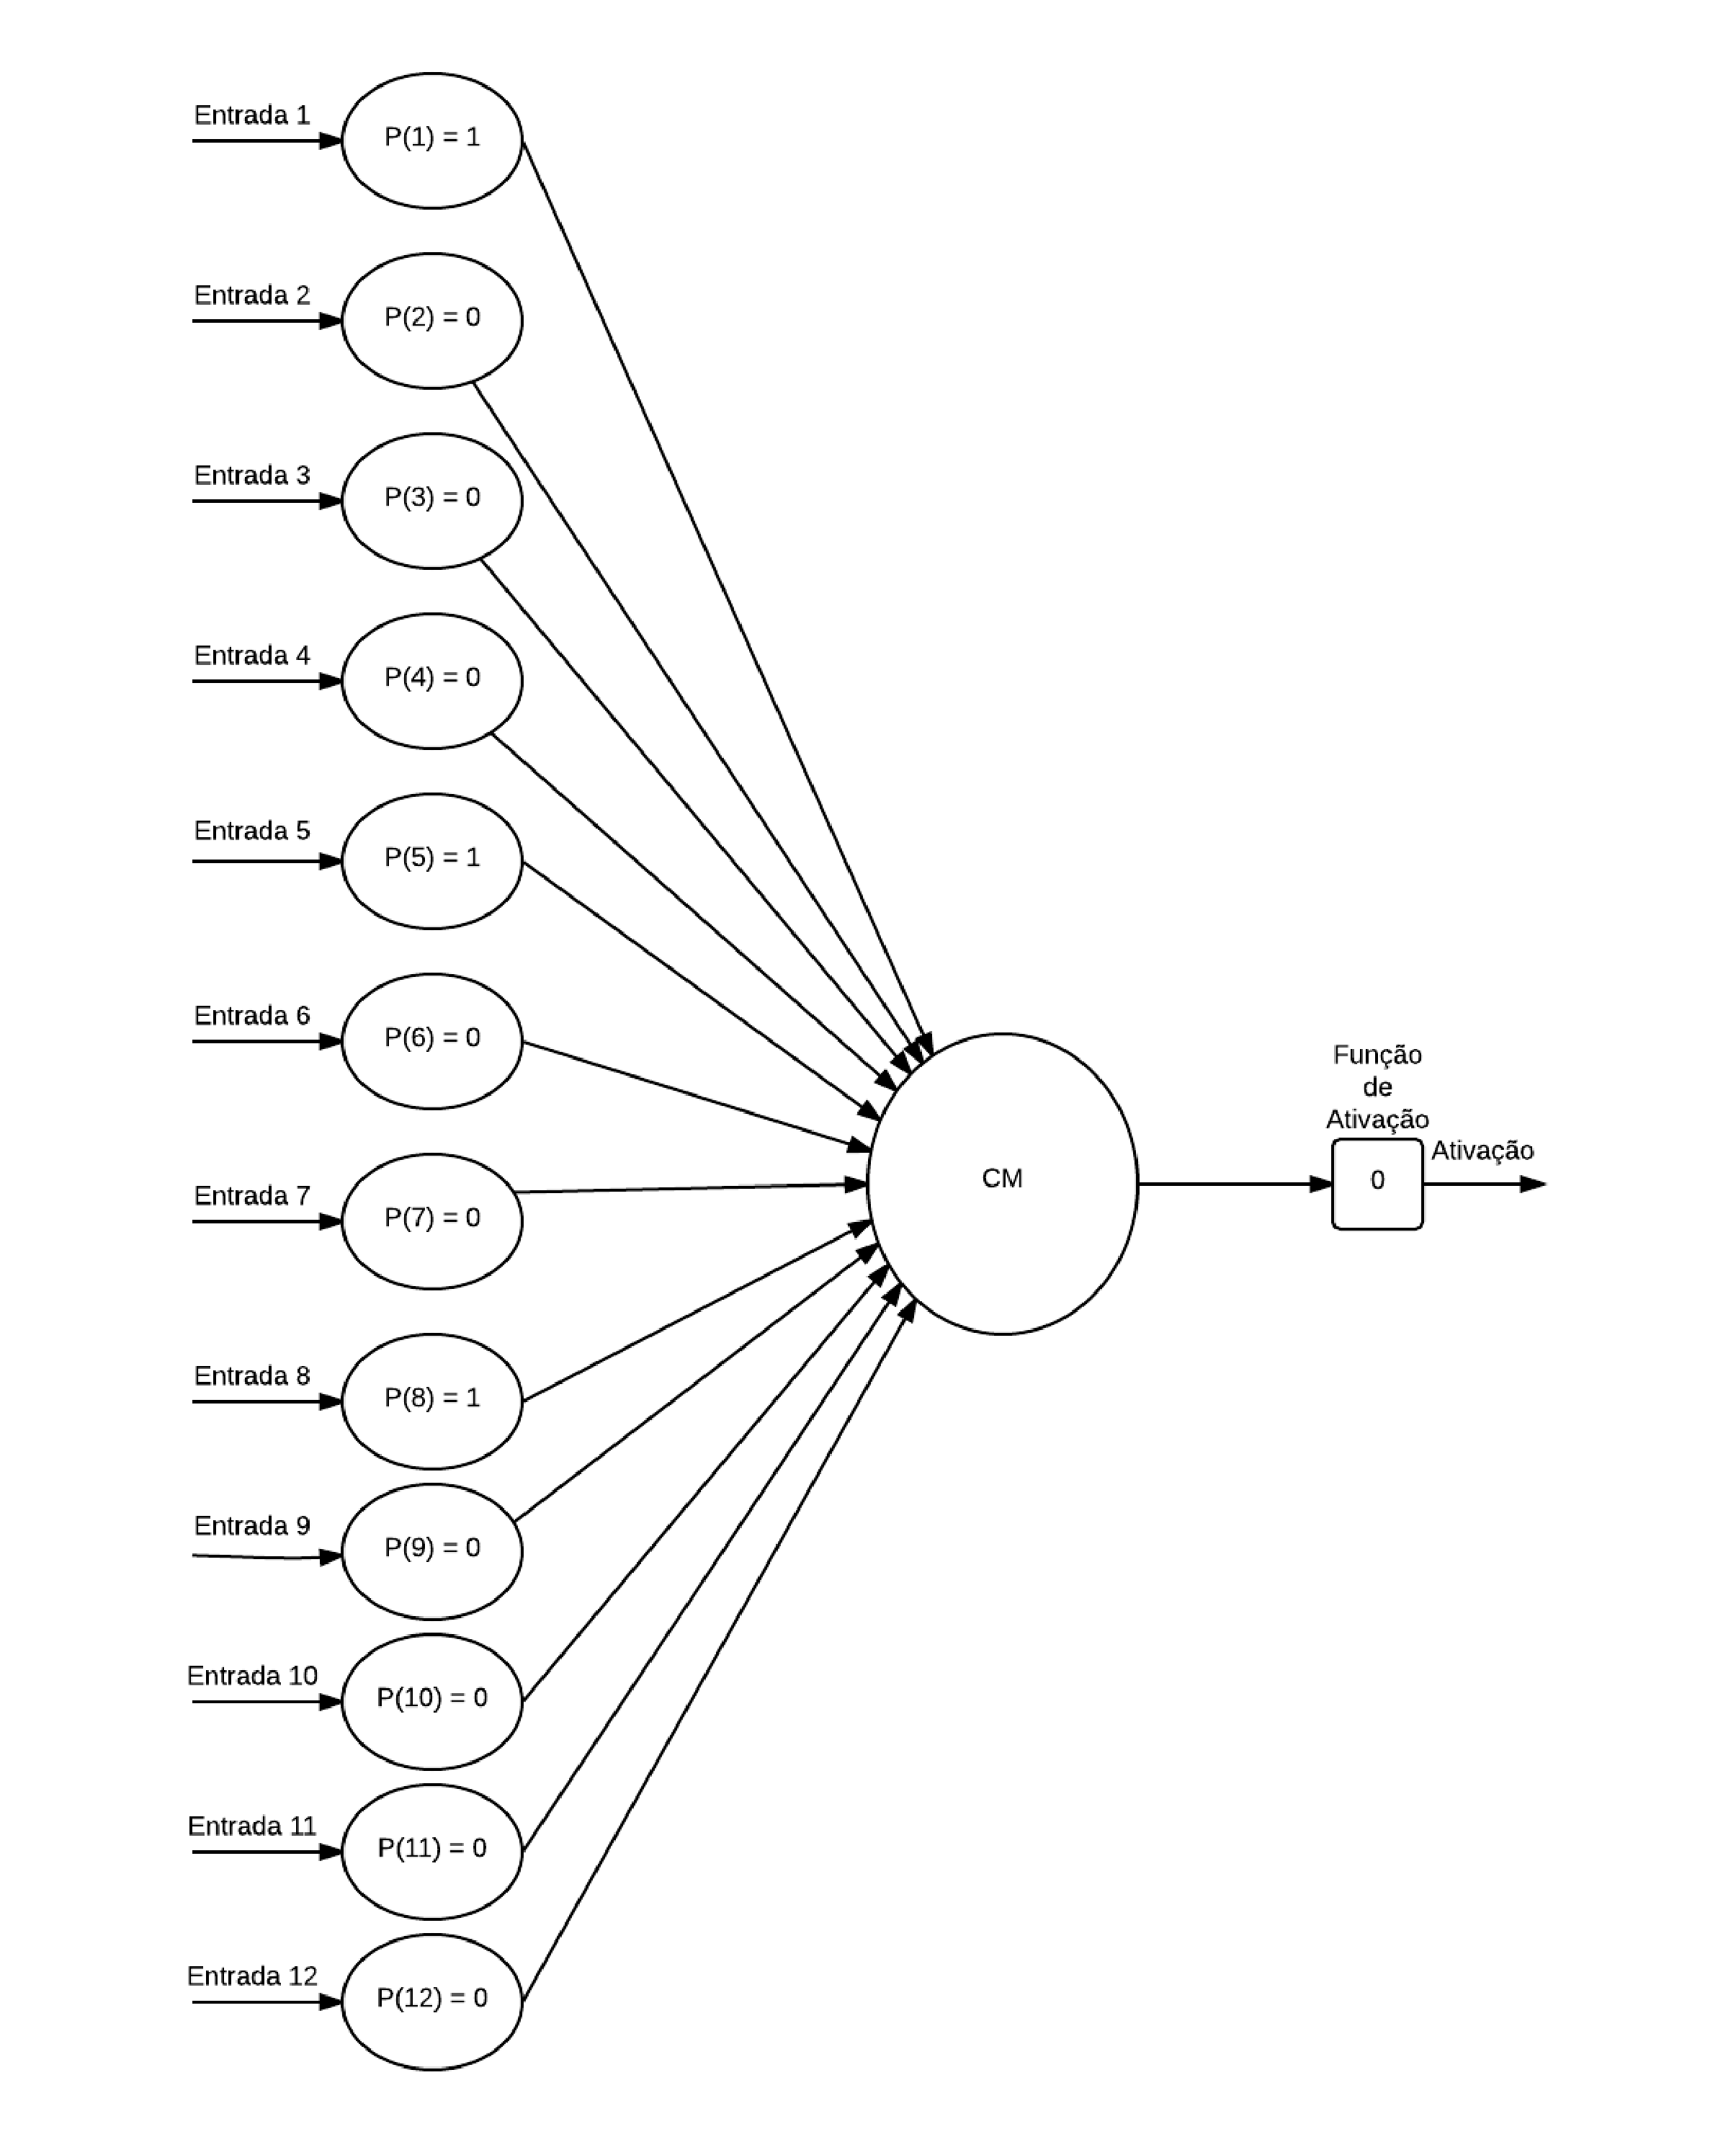
\includegraphics[keepaspectratio=true,scale=0.25]{figuras/neuron_chord}
	\caption{Esquema de Neurônio para Acordes}
\end{figure}


\newpage
Segue código para a rede neural de sugestão de acordes. Assim como a rede neural de notas, a cada iteração há o cálculo da correlação das notas sugeridas com as notas presentes nos acordes já registrados. Os procedimentos podem ser verificados abaixo:

\begin{lstlisting}
function S2 = correlate_with_chords(S1)
	exec correlation.sci;
	i = 1;
	while (i <= 48)
	     correlacao = coeffcorr(S1,BD(:,i)');
	     S2(i) = sqrt(correlacao^2);
	    i = i + 1;
	end
endfunction
\end{lstlisting}

\section{Extração do Acorde}
\label{sec:extracaoacorde}

Para a extração do acorde surgiu a necessidade de implantação da ultima camada da rede. Essa camada é chamada de classificador com máximo, ou seja, ela seleciona o valor máximo entre os impulsos do neurônios. A implementação do classificador de máximos está referenciado na seção A.8 do apêndice.

A nível de arquitetura final da rede neural, segue a ilustração:

\begin{figure}[h]
	\centering
		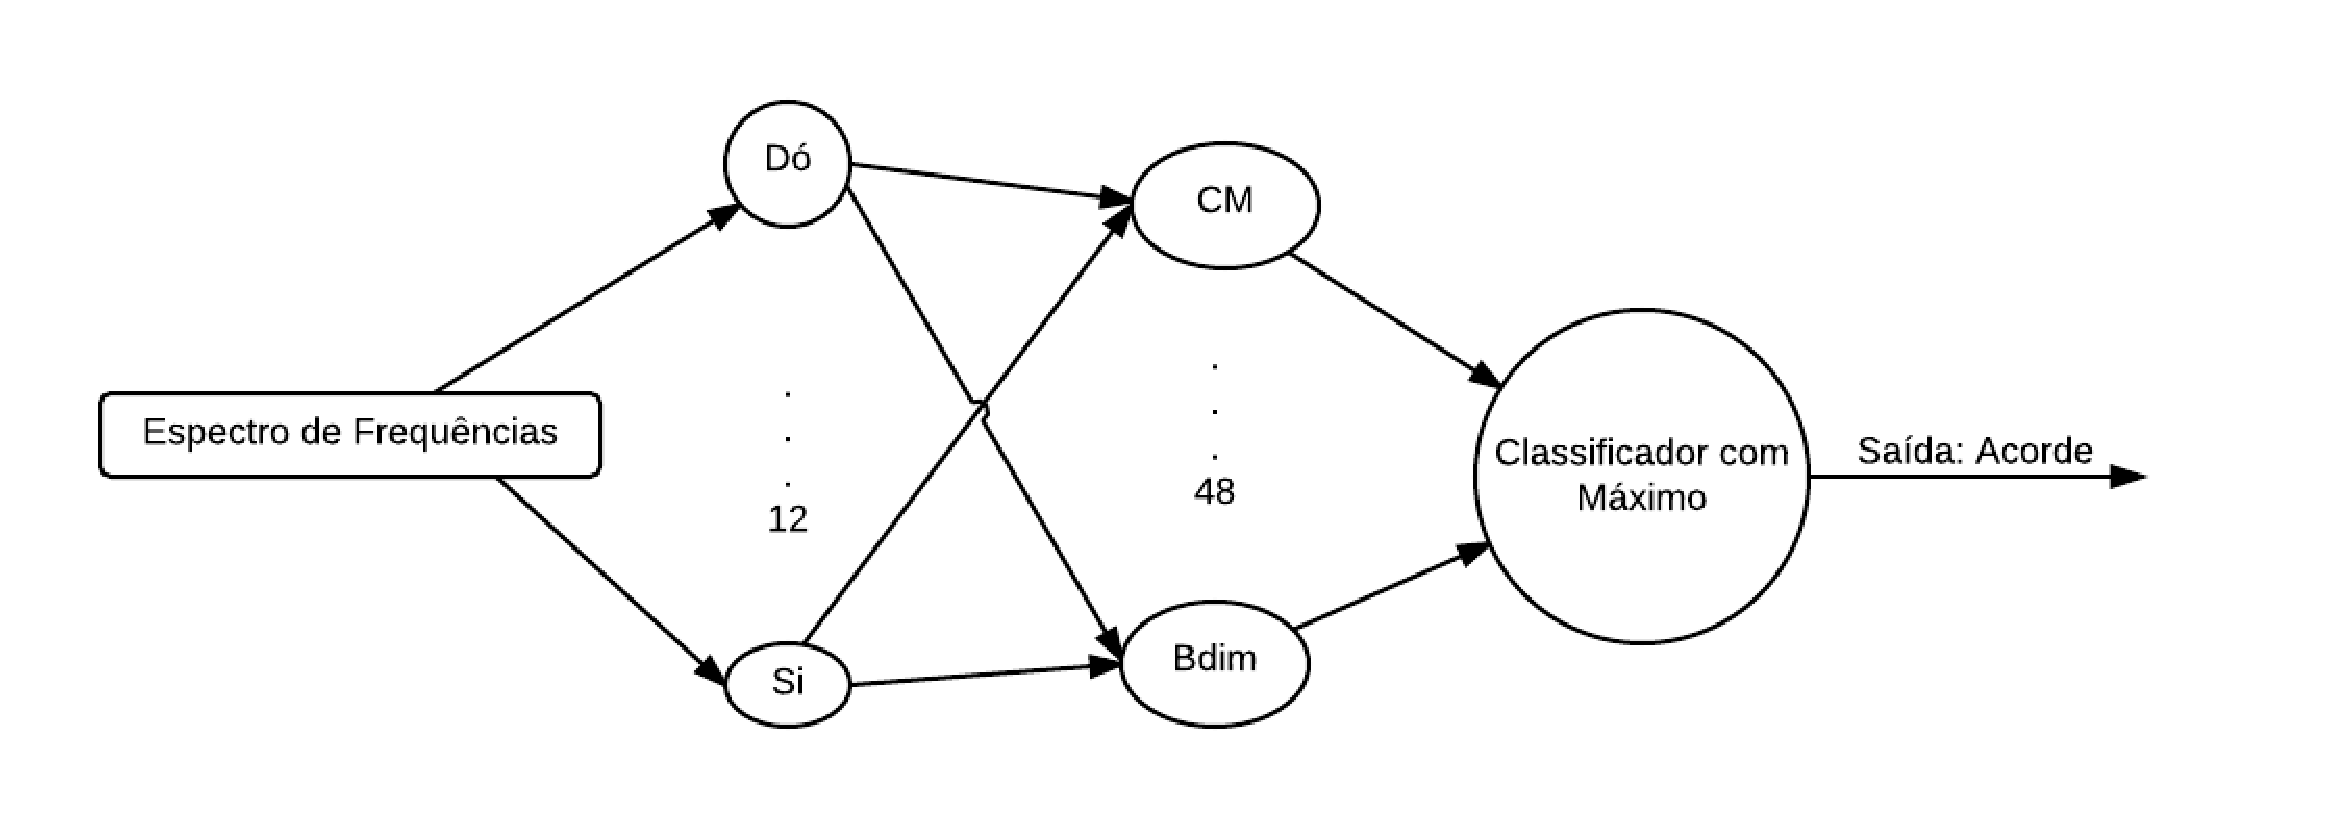
\includegraphics[keepaspectratio=true,scale=0.45]{figuras/rede_total}
	\caption{Esquema da Arquitetura Final da Rede}
\end{figure}

Em tese ela foi embasada na rede neural PNN (Probabilistic Neural Network), porém existem algumas diferenças que foram fundamentais a serem implementadas por conta do contexto. A primeira delas é que a função de transferência de todos os neurônios implementados é uma equação de correleção, pois essa função de transferência se mostrou mais sensível que o a distância euclidiana proposta no modelo padrão, visto que a correlação se embaseia na multiplicação de valores de cada vetor a ser comparado e a distância euclidiana se embaseia numa subtração (para valores pequenos a diferença é muito pequena, ao contrário da multiplicação). Ou seja, a diferença é que as 2 primeiras camadas são padrões em vez da segunda camada ser de soma dos impulsos dos neurônio da camada anterior.
